\documentclass[ieee]{uob-thesis}

\usepackage{amsmath}
\usepackage{bm}
\usepackage{eqnarray}
\usepackage{hyperref}

\usepackage{tikz}
\usetikzlibrary{arrows.meta}

\usepackage{algorithm}
\counterwithin{algorithm}{chapter}
\usepackage{algpseudocode}

\usepackage{chngcntr}
\newtheorem{remark}{Remark}
\counterwithin{remark}{chapter}

\usepackage{blindtext}
\newcommand\blfootnote[1]{%
\begingroup
\renewcommand\thefootnote{}\footnote{#1}%
\addtocounter{footnote}{-1}%
\endgroup
}

\DeclareMathOperator*{\argmax}{argmax}

\addbibresource{refs.bib}

%%%%%%%%%%%%%%%%%%%
%% AUTHOR DETAILS %
%%%%%%%%%%%%%%%%%%%


\title{Autonomous Hierarchical Control and Coordination of Unmanned Aerial Vehicle Swarms}
% \subtitle{with applications to life}
\author{Yunpeng Yang}

\DTMsavedate{thesisdate}{2024-08-31}        % do not change name, will be re-used
\date{\printdatewithoutmonth{thesisdate}}

% change as appropriate, e.g.
%   Master of Science by advanced study in Computer Science (Conversion)
%   Bachelor of Science in Computer Science
%   Master of Engineering in Computer Science
\degree{Master~of~Science~in~Computer~Science~(Conversion)}

\school{School~of~Computer~Science}
\faculty{Faculty~of~Engineering}

\wordcount{$\sim$15000}

\begin{document}

%%% -------------------------------------------------------------
%%% THESE TITLE PAGES ARE SPECIFIED BY THE REGULATIONS
%%% DO NOT CHANGE ORDER 
%%%
%%% comment out to remove any section

\maketitle
\cleardoubleoddemptypage

\begin{abstract}
In recent years, the application of unmanned aerial vehicle swarms
in civilian and military scenarios has become increasingly promising.
There has been a surge of research interest in swarm algorithms.
This thesis proposes a hierarchical swarm algorithm,
where the unmanned aerial vehicles dynamically organise themselves into a tree structure,
and coordinate with each other to carry out assigned tasks.
The algorithm enables large swarms to deal with complex tasks robustly.
The main contributions of this thesis are as follows.
\begin{itemize}
\item An application scenario of autonomous swarms is conceived (see chapter \ref{chap_problem}).
      The scenario is inspired by drone shows. The task of a swarm is to form designated shapes.
\item Based on the scenario,
      a new algorithm is designed for the hierarchical control and coordination of swarms
      (see chapter \ref{chap_design}).
\item The algorithm is implemented in the Rust programming language
      with more than 2000 lines of source code (see chapter \ref{chap_impl}).
\item Simulations are carried out
      to demonstrate the design and implementation of the algorithm (see chapter \ref{chap_sim}).
      The results show that
      the algorithm is suitable for large swarm size and complex task coordination.
\end{itemize}

Keywords: UAV swarm, hierarchical swarm, swarm control, swarm coordination.

\blfootnote{GitHub repository: \url{https://github.com/NGC0001/AutoSwarm}}
\end{abstract}

% \begin{dedication}
%   To my darling mama,\\
%   sine-qua-non.
% \end{dedication}

\begin{acknowledgements}
This thesis is accomplished under the guidance of my supervisor, Professor Ruzanna Chitchyan.
She was also one of the lecturers of the course Software Engineering.
I would like to thank her for her support and advice.
I would also like to thank all the people
who have helped me through out the year of study in the University of Bristol.
\end{acknowledgements}

\begin{declaration}
I declare that the work in this dissertation was carried out in accordance
with the requirements of the University's Regulations and Code of Practice for
Taught Programmes and that it has not been submitted for any other academic award.
Except where indicated by specific reference in the text, the work is the
candidate's own work. Work done in collaboration with, or with the assistance
of, others, is indicated as such. Any views expressed in the
dissertation are those of the author.
  
\vspace{2cm}

\includegraphics[width=4cm]{sig}
\end{declaration}

%%%
%%% TITLE PAGES END HERE
%%% -----------------------------------------------------


%%%
%% FRONT MATTER
%%%

\frontmatter

%% THESE MUST BE IN THIS ORDER ACCORDING TO REGULATIONS
\tableofcontents
\listoftables
\listoffigures


%%%%%%%%%%%%%%%%
%% MAIN MATTER %
%%%%%%%%%%%%%%%%

\mainmatter

\chapter{Aims and Objectives}
\label{chap_aim}

  Unmanned aerial vehicles (UAVs) have seen more and more application in personal life,
commercial business, industries, and military affairs.
Recently with the advance of technology, scenarios emerge where a group of UAVs
carry out an assigned task in a coordinated way \parencite{Dimakos2024, Javed2024, Ouyang2023}.
Such UAV groups are called UAV swarms.
Swarms are much more complex than individual UAVs,
and application of swarms is still in its infancy.

To fully explore and utilise UAV swarms, a lot of researchers have investigated algorithms
related to the communication, control, and task management of swarms
\parencite{Javaid2023, Zhou2020}.
Such algorithms can be roughly divided into two categories,
\textit{centralised algorithms} where a leader UAV is in charge of all the other UAVs,
and \textit{decentralised algorithms} where all UAVs are treated equally.
Decentralised algorithms can further be divided into two types,
\textit{negotiation-based algorithms} where each UAV negotiates with other UAVs to make decisions,
and \textit{reaction-based algorithms} where UAVs achieve collective behaviour through
observing other UAVs and reacting according to preset rules.

Centralised algorithms are simple,
but are prone to single points of failure induced by the leader.
Reaction-based algorithms are robust,
but are not suitable for complex tasks where elaborate coordination among UAVs is necessary.
Negotiation-based algorithms are powerful,
but entails a large amount of computation and all-to-all communication during negotiation,
effectively limiting the size of the swarm.

The \textbf{aim} of this thesis is
to \textit{find a robust algorithm suitable for large swarms and complex tasks}.
The proposed \textbf{solution} is
a \textit{hierarchical swarm} where UAVs dynamically organise themselves into a tree structure.
Instead of all-to-all communication, messages are mainly sent between UAVs
whose corresponding tree nodes are directly connected.
Tasks are managed in a divide-and-conquer way layer by layer down the tree.

To achieve this aim, the thesis below presents the following contributions:
\begin{enumerate}
    \item Firstly a \textit{swarm application scenario} is conceived (see chapter \ref{chap_problem}).
    \item Then based on the scenario,
          the \textit{algorithm is proposed} (see section \ref{sec:alg_design}),
          and the \textit{software architecture} that embodies this algorithm is \textit{designed}
           (see section \ref{sec:sft_arch}).
    \item Thirdly, a detailed \textit{implementation is built}
          to demonstrate the viability of the proposed solution (see chapter \ref{chap_impl}).
    \item Lastly,
          \textit{simulation is carried out to evaluate the algorithm} (see chapter \ref{chap_sim}).
          The results verified that the algorithm is suitable for large swarms and complex tasks. 
\end{enumerate}

\chapter{Background and Context}
\label{chap_bg}

  % two ways to ciet:
%  \textcite{label}
%  \parencite{label}

UAVs have been widely used for personal, commercial,
industrial, academic, and military purposes.
In many situations, they provide flexible and cost-effective solutions.
For example, first-person view (FPV) drones are widely used by video bloggers,
and surveillance drones greatly promote intelligence capabilities of an army.

However, the use of a single UAV is limited by its size,
sensors, computing power, and other hardware restrictions.
Besides, once a single UAV fails, the task being executed by it will also fail.
In recent years, with the advancement of technology,
it has become possible to group multiple UAVs into a swarm to perform complex tasks.
Compared to single UAVs, swarms feature the advantages of high efficiency and robustness,
and significantly expand the ways in which UAVs are used.
Many researchers have investigated the potential use cases
of swarms \parencite{Dimakos2024, Javaid2023, Ouyang2023, GAO2023, Zhou2020}.
In civilian fields, swarms can contribute to large-scale environmental monitoring,
efficient post-disaster search and rescue, forest fire fighting, logistics, etc.
In military fields, swarms may be used to enhance reconnaissance,
or even aerial warfare.

It should be noted that, a ``swarm" in this thesis refers to a group of UAVs
which autonomously coordinate with each other in real-time to complete tasks.
If the UAVs in a group just fly and operate according to preprogrammed data,
of if the UAVs are fully controlled by a remote control centre, e.g., a GCS,
then the UAV group is not considered a swarm.

Generally, for a single UAV,
the onboard hardware and software may include the following functionalities.
\begin{itemize}
    \item Communication:
    A UAV needs to exchange data with other UAVs or with a ground control station (GCS).
    \item Environment perception:
    A UAV needs to detect obstacles and to track targets.
    It also needs positioning information, which may come from a GPS receiver.
    \item Path planning:
    The flight path shall meet the requirement of a certain task.
    Collision with obstacles or other UAVs must be avoided.
    \item Flight control:
    With planned flight path, the actuators and engines shall be controlled
    according to aerodynamic principles, so as to acquire desired attitude and velocity.
    \item Task planning:
    When assigned a task, e.g., delivering a parcel,
    a UAV needs to figure out how to accomplish it.
    This is especially important for an autonomous UAV.
\end{itemize}
For a UAV swarm, except for all the above technical difficulties for single UAVs,
there are also additional challenges including
but not limited to \parencite{Javed2024, Zhou2020, Brambilla2013}:
\begin{itemize}
  \item Network topology
  \parencite{Javed2024, Javaid2023, Chen2020, Campion2019, Brust2015}:
  In some cases, the communication among UAVs is limited by a lot of factors,
  such as communication range, bandwidth, obstacles and terrain.
  An all-to-all communication network may not be feasible.
  Therefore, a good network topology design is needed to ensure efficient data transfer.
  \item Formation control
  \parencite{Javed2024, Wan2023, Ouyang2023, Shahzad2023, Ma2022, Kamel2020}:
  UAVs need to stay together to form a swarm.
  In some cases, the UAVs also need to maintain their relative positions inside a swarm.
  \item Path planning
  \parencite{Javed2024, Dimakos2024, PuenteCastro2022}:
  For swarms, the fight path needs to be planned with a view of the entire swarm.
  Besides, flight path of each individual UAV is closely coupled with
  the formation control and network topology of the whole swarm.
  \item Task planning and allocation
  \cite{Cao2024, Javed2024, Li2023, Peng2021, Ma2022}:
  The task of the whole swarm must be planned and
  divided into sub-tasks for each individual UAV.
  For most UAV tasks, task management may overlap with path planning and
  formation maintaining to some extent. For instance, in aerial search tasks,
  flight path must ensure coverage of target areas.
  While in drone shows, the task itself is to form certain formations.
\end{itemize}
To fully explore and utilise UAV swarms,
a lot of algorithms have been developed regarding different aspects of swarms.
This thesis will particularly focus on formation control and task allocation.

\section{Formation Control}

For a swarm to function normally, UAVs need to stay close to each other,
in order to communicate and cooperate.
For certain tasks, UAVs are even required to keep rigid relative positions.
Since swarm formation is ultimately achieved by the movement of every individual UAV,
formation control is therefore closely coupled with path planning.
In this section, some popular algorithms related to
formation control and path planning are reviewed.

\subsection{Leader-follower Method}

In the leader-follower method \parencite{Ouyang2023, Wan2023, Kamel2020},
one UAV is chosen as the leader, while all other UAVs are followers.
The leader is responsible for calculating the flight path.
The followers just track and follow the leader.
This method is simple to implement.
Especially for the followers,
the formation problem is converted into a trajectory tracking problem.
However, swarms employing this method risk single points of failure.
As the leader UAV acts as a central control node,
once it breaks down, the whole swarm may malfunction.
Moreover, the calculation of the swarm flight path is done by the leader alone,
which may pose a huge burden for its computing resource.

\subsection{Virtual Structure Method}

The virtual structure method treats the desired formation as a rigid virtual structure
\parencite{Ouyang2023, Wan2023, Kamel2020}.
Each UAV is expected to embody a respective virtual point on the virtual rigid body.
It observes the positions and velocities of other UAVs,
fits the position, orientation, and velocity of the virtual structure,
and then calculates its appropriate position and velocity.
There is no central UAV,
but the virtual geometric centre can be viewed as the leader of the swarm,
and all the UAVs follow this virtual leader,
as depicted by figure \ref{fig:virtual_structure}.
Therefore this method is also known as virtual leader method.

\begin{figure}[htbp]
  \centering
  \includegraphics[width=0.4\linewidth]{rsc/virtual_structure_method.png}
  \caption[Virtual structure method.]
  {In virtual structure method, the UAVs can be viewed as
  following the virtual geometric centre.}
  \label{fig:virtual_structure}
\end{figure}

Due to the elimination of a central node, the virtual structure method is robust.
But the UAVs are required to maintain a rigid formation,
this compromises flexibility in some cases, e.g., when avoiding obstacles.

\subsection{Behaviour-based Method}

Inside a swarm, each UAV may have several prescribed basic behaviours.
For eaxample, aggregation, separation, collision avoidance, and target tracking.
Each behaviour calculates a desired velocity according to some rule.
A coordinator is responsible for synthesising the final velocity out of these
behavioural velocities, based on information from the environment and other UAVs.

One of the velocity synthesis methods is the null-space
method \parencite{Arrichiello2010, Falconi2008, Antonelli2005, Bishop2001}.
Each basic behaviour is assigned a priority.
Velocity vector of lower-priority is projected onto the null space
of the immediately higher-priority velocity, as shown in figure \ref{fig:null_space}.
In this way, lower-priority behaviour will not conflict with higher-priority behaviour.

\begin{figure}[htbp]
  \centering
  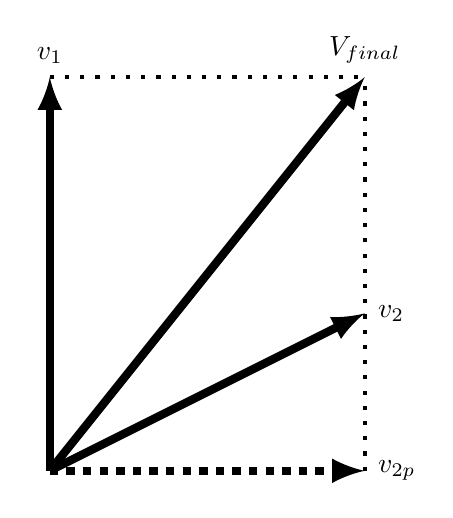
\begin{tikzpicture}
    \draw[line width=3pt,black,-latex](0,0)--(0,5) node[anchor=south]{$v_1$};
    \draw[line width=3pt,black,-latex](0,0)--(4,2) node[anchor=west]{$v_2$};
    \draw[line width=3pt,black,dashed,-latex](0,0)--(4,0) node[anchor=west]{$v_{2p}$};
    \draw[line width=1.5pt,black,loosely dotted](4,0)--(4,5);
    \draw[line width=1.5pt,black,loosely dotted](0,5)--(4,5);
    \draw[line width=3pt,black,-latex](0,0)--(4,5) node[anchor=south]{$V_{final}$};
  \end{tikzpicture}
  \caption[Null-space method.]
  {In null-space method, the velocity $v_2$ from the lower-priority behaviour
  is projected onto the null space of the higher-priority $v_1$,
  resulting in $v_{2p}$, and the final velocity is $V_{final} = v_1 + v_{2p}$.}
  \label{fig:null_space}
\end{figure}

Behaviour-based method can be used not only in UAV swarm
formation control and path planning, in fact, it can be viewed as a
general framework for coordinating interacting behaviours \parencite{Kamel2020}.
The behaviour coordination mechanism is at the core of this method.
For the case of formation control, behaviour coordination means velocity synthesis.

\subsection{Bio-inspired Methods and Other Methods}

Bio-inspired methods draw ideas from natural swarm behaviours,
especially biological phenomena.
For example, many bird species fly in flocks,
so if UAVs imitate the behaviours of birds, UAV swarms may display similarities to
bird flocks \parencite{Ma2022, Reynolds1987}.
Another interesting example is morphogenesis approach \parencite{Ma2022, MAMEI2004}.
Morphogenesis, i.e., the formation of the shape of organs,
is connected with signal molecules that diffuse among cells, also known as morphogen.
Cells adjust their behaviour according to the concentration of morphogen,
and eventually the organ will develop a certain shape.
Inside a swarm, messages can be propagated in certain pattern between neighbouring UAVs.
If all UAVs act properly according to these messages,
the swarm will be able to develop a global shape in a self-organised way.

There are also many other types of formation control methods,
such as artificial intelligence (AI) methods \parencite{PuenteCastro2022},
artificial potential fields \parencite{Shahzad2023, Wang2006, Schneider2003},
graph-based(consensus-based) algorithms \parencite{Ouyang2023, Kamel2020},
and so on.

\section{Task Allocation}

However, for an autonomous swarm,
it is equally crucial to optimally schedule tasks and allocate them to individual UAVs.
Usually, for UAV, task management is highly related to path planning,
after all, most tasks have restrictions on the position and velocity of a UAV.
Moreover, in real scenarios, resources such as fuel or power are constrained for a task,
making the problem even harder to tackle \parencite{Javed2024, Zhou2020}.

One relatively easy way to manage swarm tasks is to take a centralised approach.
That is, one UAV works as a central node, schedules tasks and allocates them to others.
However, due to single points of failure, this method is not robust.
Decentralised methods, where every UAV takes part in the task allocation process,
are more resilient but also more complex.
Many algorithms have been studied for their usage
in swarm task allocation \cite{Peng2021, Plathottam2018},
such as game theory, reinforcement learning, etc.
In this section, some of them are reviewed.

\subsection{Algorithms Based on Market Mechanisms}

These algorithms imitate marketing processes.
A typical example is the auction algorithm \parencite{Peng2021, Kim2020, Sujit2007}.
If a UAV has a task, but does not own the requisite resource,
it can choose to auction the task.
Other UAVs can bid, and the winner is assigned the task.
Auction algorithm has clear rules and is easy to perform.
It requires good communication between the auctioneer and the bidders.

\subsection{Consensus-based Methods}

In consensus methods, if a UAV wants to take any action,
or if it wants the whole swarm to take any action,
it firstly negotiates with other UAVs,
and they need to reach an agreement on whether or not the action should be taken.
If consensus is reached, the action will be taken,
otherwise the action is abandoned.
It can be seen that consensus algorithms require good communication inside the swarm.
Many researchers have studied different types of consensus methods and
their variants \parencite{Pasek2022, Ranganathan2022, Grishchenko2021, Li2019}.
The difficult part of a consensus algorithm is for a UAV to decide
whether all others have been informed of and have agreed on its proposal,
especially in real-world scenarios where network topology is constrained
and communication condition is not ideal.

Consensus algorithms have a wide range of applications.
They can be used not only in swarm task allocation,
but also in formation control, path planning,
and many other types of distributed systems,
e.g., a distributed software system \parencite{Ongaro2014}.

\subsection{Optimisation Algorithms}

Since time and resources are limited for a swarm,
optimisation algorithms come into play,
so as to plan and allocate tasks in a most optimal way.
Note that, optimisation is not used for
reaching an agreement on which UAV takes which sub-task,
but for finding out the best task division scheme.

A particular type of optimisation methods are swarm intelligence algorithms
\parencite{Cao2024, Javed2024, Tang2023, Peng2021, Zhou2020, Tan2013, Beni1993}.
Swarm intelligence is not a strict term,
but a loose concept that solves problems by modelling a population of agents
which can self-organise and interact with each other.
After a population is set to some initial state,
each individual agent acts by certain principle,
eventually, the whole population may achieve specific collective behaviour
or reach desired global optimum state.
A lot of swarm intelligence methods are inspired by biological swarm behaviours.
Swarm intelligence can be used in many problems, and optimisation is just one of them.
Some common swarm intelligence optimisation algorithms are genetic algorithm (GA),
particle swarm optimisation (PSO) \parencite{Bonyadi2017, Duan2013, Roberge2013},
ant colony optimization (ACO),
wolf pack algorithm (WPA) \parencite{Xu2022, Lu2020},
and so on.

\section{Hierarchical Swarm}

Despite of lot of research effort put into UAV swarms,
they are still not mature for real-world applications.
In 2021, \textcite{Lee2021} reported an experiment where
3 UAVs planned their flight path to avoid no-fly zones and
kept their formation with leader-follower method.
In 2016, US department of defense conducted a micro-drone swarm test \parencite{DOD2017}.
In the test, 103 small drones were launched from fighter jets.
The drones demonstrated collective decision making,
adaptive formation flying, and other swarm behaviours.
However, technical details were not disclosed.
In 2022, British Army carried out a demonstration where
swarms comprised of 4 or 6 drones executed autonomous missions \parencite{BA2022}.
Again, no technical details.
As can be seen from the above examples,
current swarms are either quite small, or can only deal with simple tasks.
This is not surprising since swarm algorithms are still in their early stage.

\subsection{Drawbacks of Common Algorithms}

Swarm control algorithms can be roughly divided into two categories,
centralised ones and decentralised ones.
Centralised algorithms usually have a leader UAV as a central node,
whereas all other UAVs are managed by the leader.
The leader-follower formation control method is an example of centralised algorithm.
Such algorithms are simple and efficient,
but are vulnerable to single points of failure.
Besides, as most computation happens on the central node,
it usually needs much more communication and computing power than others.
Therefore the swarm size may be limited by the resource on the central node.
In contrast, decentralised algorithms treat every UAV equally,
and the collective behaviour of the whole swarm is coordinated by all the UAVs involved.
Such algorithms are more robust.

In this thesis, decentralised algorithms are further divided into two types.
The first type is negotiation-based ones,
such as auction algorithms and consensus algorithms.
UAVs communicate with each other about what they plan to do next,
and make decisions together.
Consensus algorithms are powerful,
because each UAV knows what others will do,
and they have a fine control on task management.
However, they impose a high communication and computation burden on swarms,
since every UAV cares for the whole swarm.
As swarm population increases,
the complexity of communication and control goes up sharply.
Thus, the swarm size is limited.

Another type of decentralised algorithms is reaction-based ones,
such as virtual structure formation control, and most bio-inspired algorithms.
In these algorithms, UAVs do not need to reach agreement.
They just gather information about the environment and other UAVs,
then they react according to preset rules.
Such algorithms are highly robust,
and do not require much communication or computation resource.
They are highly distributed and suitable for large swarms.
However, they lack fine and flexible control over the swarm,
hence are not versatile and are only adequate for simple tasks.
Table \ref{tbl:algorithms_cmp} shows a comparison between different types of algorithms.

\begin{table}[htbp]
\centering
\caption[Comparison of swarm algorithms.]
{Comparison of different types of swarm algorithms.}
\label{tbl:algorithms_cmp}
\begin{tabular}{|c||c|c|c|}
  \hline
  Algorithm Type       & Centralised         & Negotiation-based & Reaction-based \\
  \hline\hline
  Robustness           & not robust          & robust            & robust         \\
  \hline
  Algorithm Complexity & simple              & complex           & intermediate   \\
  \hline
  Performance Overhead & high (central node) & high (all nodes)  & low            \\
  \hline
  Supported Tasks      & complex             & complex           & simple         \\
  \hline
  Supported Swarm Size & small               & small             & large          \\
  \hline
\end{tabular}
\end{table}

\subsection{A Hierarchical Method}

This thesis aims to find an algorithm that is robust, suitable for complex tasks,
adequate for large swarms, and low in performance overhead.
The solution is a hierarchical swarm.
The swarm is organised into a tree structure.
Each UAV corresponds to a node on the tree structure,
and it is in direct control of the UAVs which correspond to its child nodes.
Layer by layer, the root node will be controlling the whole swarm in an indirect way,
quite similar to the hierarchy in modern companies, governments, or armies.
Figure \ref{fig:swarm_tree} shows such an swarm structure.
Communication mainly happens between each parent-child node pairs.
For most of the time, there is no need for many-to-many communication,
reducing the communication overhead.
Task is also solved by hierarchical coordination.
A node receives task from its parent, then divides the task,
and assigns the sub-tasks to itself and its children.
The children then repeat the process.
This divide-and-conquer way of task coordination potentially reduces computing overhead.
As the tree grows in depth, the number of nodes grows exponentially,
therefore large swarm sizes are supported.

\begin{figure}[htbp]
  \centering
  \includegraphics[width=0.4\linewidth]{rsc/swarm_tree.png}
  \caption[Hierarchical swarm.]
  {A swarm organised hierarchically into a three-layer tree.
  Arrows point from parent node to child node.}
  \label{fig:swarm_tree}
\end{figure}

Actually, researchers have already investigated the usage of hierarchical structure
in swarm organisation \parencite{CHEN2021, Wang2021, Tahir2020}.
In those researches, the hierarchy, which is not necessarily a tree,
is predefined and fixed before flight.
This leads to reduced flexibility and robustness.
In fact, a tree is just a multi-layered leader-follower structure, which is centralised.
To mitigate the disadvantages of leader-follower approach induced by centralisation,
some researchers have proposed dynamic leader election
algorithms \parencite{Ganesan2020, Brust2015}.
Similarly, to make the swarm tree structure flexible and robust,
it needs to be organised dynamically.
That is, the UAVs themselves build up the tree,
and they are able to repair the tree structure in case any of them fails.

In the next chapters, the algorithm for dynamic hierarchical swarm organisation
will be developed and implemented.
The task for the swarm is to form designated geometric shapes.
This application scenario is inspired by drone light shows \parencite{VergeAero}.
Currently, drone light shows do not employ autonomous UAV swarms.
But this thesis shows the possibility for their usage in the future.

\chapter{Problem Formulation}
\label{chap_problem}

  To develop and demonstrate a swarm algorithm,
an application scenario is needed.
Inspired by drone shows, where drones form various interesting shapes,
in this thesis, the task for a swarm is to form a designated geometric shape.
Since the purpose is focused on swarm control and coordination, many other aspects,
such as aerodynamics, obstacle avoidance, and power or fuel management,
are ignored or simplified.
The problem is formulated below.

\section{UAV Properties}

At time point $t = 0$, a set of homogeneous UAVs
$W = \{U_i | i = 0, 1, \ldots, N_u-1; N_u > 0\}$
are located at initial positions $\bm{P}_i(t=0) = (x_{i0}, y_{i0}, z_{i0})$.
They are already airborne. The taking-off process is not considered.

Each UAV $U_i$ has a unique ID $id_i$.
The ID set has total order, which means IDs are comparable.

GPS receivers are installed, so UAVs can read
their positions $\bm{P}_i(t) = (x_i, y_i, z_i)$.
The distance between two UAVs $U_i$ and $U_j$ is
\begin{equation}
d_{ij}(t) = d_{ji}(t) = ||\bm{P}_i(t) - \bm{P}_j(t)||.
\end{equation}
They will clash if $d_{ij} \leqslant 2 r_{rad}$,
where $r_{rad}$ is the radius of a UAV.

UAVs are able to move at arbitrary velocity $\bm{V}_i(t) = (vx_i, vy_i, vz_i)$,
as long as
\begin{equation}
v_i(t) = ||\bm{V}_i(t)|| \leqslant v_{max},
\end{equation}
where $v_{max}$ is the given maximum speed of the UAVs.
Hovering, i.e., $\bm{V} = \bm{0}$, is allowed.
In real cases, a UAV can only control its engines or rotors.
The actual acceleration and velocity are determined by engine power and aerodynamics.
In this thesis, the flight control is greatly simplified,
and the UAVs are assumed to be able to change their velocity directly.
Besides, it's assumed that the UAVs fly in the same manner in all directions,
without the need to care about attitude,
which is of course not true for any real UAVs.

UAVs do not known the existence of each other at $t = 0$.
UAV $U_i$ can receive all the data sent by UAV $U_j$
if the distance between them is within the given communication range $r_{comm}$,
i.e., $d_{ij} \leqslant r_{comm}$.
Latency and bandwidth problems are not considered.
At $t = 0$, the initial positions of the UAVs ensure that,
any two UAVs are within communication range.

\section{Representation of Geometric Shapes}

A ``shape" here is made up of one or multiple lines.
While a ``line" here is made up of one or multiple connected line segments.
A line segment is defined by two points,
so a line can be defined by a sequence of points.

Let $L$ represent a sequence of $N_p$ different points
$\bm{P}_0, \bm{P}_1, \ldots, \bm{P}_{N_p-1}$,
where $\bm{P}_k = (x_k, y_k, z_k), 0 \leqslant k \leqslant N_p-1$,
and $N_p \geqslant 2$.
$L$ defines $N_p - 1$ connected line segments, which form a ``line".
A point $\bm{P} = (x, y, z)$ is said to be on line $L$
if it falls onto any of the line segments,
that is, there exist an integer $i, 0 \leqslant i < N_p-1$,
and a real number $c, 0 \leqslant c \leqslant 1$, such that
\begin{eqnarray}
    (x - x_i) &=& c(x_{i+1} - x_i), \\
    (y - y_i) &=& c(y_{i+1} - y_i), \\
    (z - z_i) &=& c(z_{i+1} - z_i).
\end{eqnarray}
A shape $S$ is a set of $N_l$ lines $\{L_m | m = 0, 1, \ldots, N_l-1; N_l > 0\}$.
$\bm{P}$ is said to be on $S$ if it is on any of the lines.

Lines defined above can not represent curves.
However, a curve can be approximated by a large amount of short line segments,
in the commonly used way how a circle is approximated by a polygon.

\section{Swarm Tasks}
\label{sec:swm_tsk}

A task $TSK$ contains a unique task ID $tid$, a shape $S$ and a time period $\Delta t$.

Let $W$ be a set of UAVs.
At some time point $t'$,
task $TSK$ is sent by GCS to an arbitrary member of $W$.
The mission for $W$ is,
all the UAVs move onto the shape and stay for $\Delta t$.
That is, the task is said to be successfully executed
if there exists a time point $T, t' \leqslant T < +\infty$,
such that for any time point $t \in [T, T+\Delta t]$ and for any UAV $U \in W$,
$U$ is on $S$.

Collisions shall be avoided.
That is, at any time point $t$, for any two UAVs $U_i$ and $U_j$,
the distance between them shall satisfy $d_{ij} > 2 r_{rad}$.

Additionally, UAVs should be distributed as evenly as possible along the lines.
This means to minimise the mean square root of UAV intervals along the lines.
This is not the primary goal of the task, so it is not formally stated here.
But later in section \ref{sec:tsk_div},
an algorithm will be implemented to address this goal.

\chapter{Algorithm and Software Design}
\label{chap_design}

  In this chapter, the swarm algorithm is shown step by step
to solve the problem stated in chapter \ref{chap_problem}.
The module-level architecture of the onboard software based on this algorithm
is also designed and detailed.

\section{Swarm Algorithm Design}
\label{sec:alg_design}

\subsection{Dynamic Organisation of Tree Structure}

Before a group of UAVs is able to handle any task,
the UAVs should firstly organise themselves into a tree structure.
Since each UAV can be viewed as a single-node tree,
the problem can be viewed as building a single large tree from all existing small trees.
Before continuing, some terms, assumptions and key designs must be clarified.
\begin{remark}
    A swarm is defined as all the UAVs on the same tree.
    A sub-swarm is defined as all the UAVs on a sub-tree.
\end{remark}
In the context of this thesis, the term ``tree" is equivalent to the term ``swarm",
and they will be used interchangeably.
Similarly, term ``node" is sometimes used to refer to a UAV inside a swarm.
Building a single tree from small trees means building a single swarm from existing small swarms.
\begin{remark}
    Inside a tree, each child-parent node pair forms a connection.
    The child shall ensure that its distance from the parent is within communication range.
\end{remark}
A node may be in connection with multiple child nodes, but with at most one parent node.
For each child-parent pair, the child needs to track the parent
since it is responsible for keeping the communication range.
\begin{remark}
    Child node and parent node send connection messages to each other periodically,
    in order to exchange necessary data.
\end{remark}
To distinguish from the root UAV of the whole tree,
the root node of a sub-tree will be called the top node of that sub-tree.
\begin{remark}
    Inside a tree, for each child-parent node pair,
    the sub-tree topped by the child node is called a ``child sub-tree" of the parent node.
\end{remark}
\begin{remark}
    The size of a tree is the number of its nodes, i.e., the population of the swarm.
\end{remark}
\begin{remark}
    A set of existing trees can be strictly ordered by tree size and root node UAV ID.
\end{remark}
Trees of different sizes can be ordered by size.
Since UAV IDs are unique and comparable,
two trees of the same size can be distinguished and ordered by root node UAV ID.
\begin{remark}
    For a node on a tree, the ID sequence of all its ancestor nodes and itself
    is called the NID (meaning ``node ID") of the node.
\end{remark}
If the root node of a tree is UAV $U_i$, $U_i$ has child $U_j$,
and $U_j$ has child $U_k$, then the NID of $U_k$ is $[id_i, id_j, id_k]$.
An NID always starts with the ID of the root node of the tree.
The root node always knows its NID.
If a parent node knows its NID and sends its NID to its children,
the children will also known their NIDs.
\begin{remark}
    If every parent node sends its NID to its child nodes,
    recursively all nodes will known their correct NIDs.
\end{remark}
For a leaf node, i.e., node that has no children,
its sub-tree size is one, since the only member of the sub-swarm is itself.
For a parent node, if all its children know their respective sub-tree sizes
and send the data to the parent node,
the parent node can then calculate its own sub-tree size,
which is the sum of child sub-tree sizes plus one.
\begin{remark}
    If every child node sends its sub-tree size to its parent node,
    recursively all nodes will known their correct sub-tree sizes.
\end{remark}
For the root node, its sub-tree size is also the size of the whole tree.
\begin{remark}
    If every parent node sends tree-size data to its child nodes,
    recursively all nodes will known the correct tree size.
\end{remark}
The ultimate purpose of a swarm is to carry out tasks assigned by GCS.
For any swarm member, it may be handling some task, or it may be in free state.
\begin{remark}
    The ``current task ID" of a UAV is denoted by the $tid$ of the task,
    or is $None$ if the UAV is free.
\end{remark}
In order for the UAVs to discover each other and to obtain the status of each other,
they need to broadcast their information to nearby UAVs.
\begin{remark}
    A UAV broadcasts its NID, position, velocity, swarm size and current task ID periodically.
\end{remark}

Now the basic characteristics of a swarm are established,
and a UAV knows well about other UAVs in its neighbourhood. 
Initially, each UAV is a single-node tree.
To build a single tree from multiple existing trees,
two ideas are feasible: swarm-merging and swarm-switching.
\begin{itemize}
  \item Swarm-merging.
  For a swarm, if there are bigger other swarms nearby,
  the root node, leading the whole current swarm, joins the biggest swarm.
  \item Swarm-switching.
  For a UAV in a swarm, if there are bigger other swarms nearby,
  the UAV, leading its sub-swarm, leaves the current swarm and joins the biggest swarm.
\end{itemize}

In swarm-merging method, a smaller tree joins a bigger tree as a whole.
Trees are stable.
Existing trees will not collapse during merging process unless failure occurs.
In swarm-switching method, trees are not stable since nodes may leave at any time.
However, it's hard for swarm-merging method to handle the case
where the nearby biggest swarm is found by a non-root node,
but is out of the communication range of the root node.
Whereas for tree-switching method,
the node which finds the biggest swarm just joins the new swarm,
and other nodes of the old swarm will almost certainly find the new swarm
since they are at least in the communication range of that switching node.

The swarm-switching method is adopted.
The pseudocode is shown in algorithm \ref{alg:swarm-switching}.
The variable $self$ in the algorithm refers to the UAV that runs the algorithm.
The algorithm is only run when a UAV is free, i.e., when its current task ID is $None$.
The root node ID is used to tell which tree a node is currently on,
it is contained in the NID of a node.
When comparing two swarms, the swarm of bigger size is ordered before the one of smaller size.
If two swarms are of the same size,
the swarm with smaller root ID is ordered before the one with bigger root ID.

\begin{algorithm}
\caption{Swarm-switching algorithm.}
\label{alg:swarm-switching}
\begin{algorithmic}[1]
\Require $self$ is free
\Function{SwitchTree}{$self$}
\State $root\_self \gets self$.get\_root\_id()
\State $candidates \gets$ all nearby UAVs
\State $candidates$.filter\_by($candidate$ is free)
\State $candidates$.filter\_by($candidate$.get\_root\_id() $\neq root\_self$)
\State $candidates$.filter\_by(swarm of $candidate$ ordered before swarm of $self$)
\If{$candidates$ is not empty}
    \State $candidates$.sort\_by(ordering of their respective swarms)
    \State $new\_swarm\_root \gets candidates[0]$.get\_root\_id()
    \State $candidates$.filter\_by($candidate$.get\_root\_id() $= new\_swarm\_root$)
    \State $candidates$.sort\_ascending\_by(distance($candidate$, $self$))
    \State $self$.set\_parent($candidates[0]$)
\EndIf
\EndFunction
\end{algorithmic}
\end{algorithm}

In algorithm \ref{alg:swarm-switching},
after a UAV $U_i$ sets another UAV $U_j$ as its parent node,
$U_i$ should send a request message to $U_j$.
$U_j$ can accept the request,
or if $U_j$ is in inappropriate state,
it can reject the request by sending $U_i$ a reject message.
If $U_i$ receives a reject message,
it separates from $U_j$ and the sub-tree led by it becomes a new independent tree.

If all free UAVs within communication range keep running algorithm \ref{alg:swarm-switching},
they will eventually form a single tree.
Due to the latency of data flow inside a tree,
information stored by a node, such as swarm size, may not be updated timely.
Theoretically, this may cause nodes to join a tree which is not the biggest one.
However, information will eventually propagate throughout a tree,
and the algorithm is expected to converge.

\subsection{Task Coordination}

Tasks are handled hierarchically.
The root node divides the shape of a task into parts,
one for itself, and the others sent to its children.
Its children then repeat this process, until every node gets a portion of the shape.
Execution of a task means adjusting the velocity appropriately,
so the UAV flies onto its part of the shape, and stays there for a required time duration.

In this thesis, based on the context, the word ``task" may refer to three cases:
the task sent by the GCS to a swarm;
a portion of the task that is allocated to a sub-swarm;
a portion of the task that is allocated to a node.
The word ``sub-task" is also used to refer to the latter two cases.

When the UAVs are in free state, the swarm is not stable.
Nodes may join or leave a swarm.
It is hard for an unstable swarm to handle tasks properly.
So after a swarm receives a task,
it needs to firstly fix itself before it starts to handle the task.
An inner state is needed for every UAV to represent whether it has a task.
\begin{remark}
    The current task ID of a UAV is none $\iff$ the UAV is in state $Free$;
    the current task ID of a UAV is some $tid$ $\iff$ the UAV is in state $InTask$.
\end{remark}
\begin{remark}
    If a UAV is in state $InTask$, it shall not leave the swarm;
    it shall also reject any request that sets it as parent.
\end{remark}
It can be seen that if all members of a swarm is in $InTask$ state, the swarm is stable.
So after a task is received,
an approach is needed to transform the whole swarm into $InTask$ state.
\begin{remark}
    Based on the execution state of the task,
    $InTask$ state has three sub-states:
    $InTask(InProgess)$, $InTask(Success)$ and $InTask(Failure)$.
\end{remark}
\begin{remark}
    If a non-root UAV receives a task message sent by GCS,
    it relays the GCS task to its parent node.
    If root UAV receives a GCS task,
    it turns from $Free$ state into $InTask(InProgress)$ state.
\end{remark}
A child node can receive the current task ID of its parent node.
It changes its state according to this information.
\begin{remark}
    A child node turns into $Free$ state if the current task ID of its parent is $None$;
    and turns into $InTask(InProgress)$ state if the current task ID of its parent is some $tid$.
\end{remark}
All UAVs in a swarm will recursively align their $Free$/$InTask$ states with the root UAV.
After the root node receives a GCS task,
the whole swarm will gradually transform into $InTask(InProgress)$ state.
Before this alignment is complete,
the tree structure may change,
besides, the swarm size and sub-swarm size data stored by a UAV may be incorrect,
so task division is not possible.
Note that, for non-root nodes,
$InTask$ means it has received the task ID,
but may or may not have actually received a sub-task.

After the root node turns into $InTask(InProgress)$,
it needs to know whether all the other UAVs have finished aligning their states,
in order to start to divide the task and allocate sub-tasks.
In addition, once a task is fully divided and allocated to every node,
the root node needs to know the sub-task results of all other UAVs,
in order to decide the final result of the task.
\begin{remark}
    A node in $InTask(InProgress)$ turns into $InTask(Success)$
    if all nodes in its sub-tree succeeded in executing the task;
    A node in $InTask(InProgress)$ turns into $InTask(Failure)$
    if any node in its sub-tree failed in executing the task.
\end{remark}

Again, those information can be collected in a recursive way.
For this purpose, besides the state of a node itself,
the overall state of the sub-tree topped by the node is also needed.
\begin{remark}
    At any time point, a sub-swarm is in one of the six task states:
    $None$, $Recv$, $Algn$, $Allc$, $Succ$, and $Fail$.
\end{remark}
The meaning of the six task states are explained in table \ref{tbl:subswm_tsk_state}.
The top node of a sub-tree is responsible for
calculating the sub-swarm task state and sending it to its parent node.
The calculation process is shown in algorithm \ref{alg:subswarm-tsk-state}.
It is seen that the top node needs data from its children to do the calculation,
which means recursion.
A leaf node has no children.
Once it receives a task ID and turns into $InTask(InProgress)$,
its sub-tree, which contains only itself, is in task state $Algn$.
The node then reports $Algn$ to its parent.
If all children of the parent report $Algn$,
the parent knows that all its child sub-trees have been aligned to $InTask$,
and the parent's sub-tree is in task state $Algn$.
Recursively, the root node will eventually know that the whole swarm has been aligned.
Sub-task results are propagated up the tree in a similar way.

\begin{table}[htbp]
\centering
\caption[Sub-swarm task states.]
{The meaning of the six task states of a sub-swarm.}
\label{tbl:subswm_tsk_state}
\begin{tabular}{c|p{0.75\linewidth}}
  \hline
  $None$ & The top node is in $Free$ state. \\
  \hline
  $Recv$ & The top node has received the task ID and is in $InTask(InProgress)$,
           but has not confirmed that all the other nodes of the sub-tree are in $InTask$. \\
  \hline
  $Algn$ & The top node has confirmed that all nodes of the sub-tree are in $InTask$,
           and it has not received a sub-task from its parent. \\
  \hline
  $Allc$ & The top node has confirmed that all nodes of the sub-tree are in $InTask$,
           and it has received a sub-task from its parent. \\
  \hline
  $Succ$ & The top node finds that all nodes of the sub-tree have succeeded. \\
  \hline
  $Fail$ & The top node finds that at least one node of the sub-tree has failed. \\
  \hline
\end{tabular}
\end{table}

\begin{algorithm}
\caption{The process of the top node calculating the sub-swarm task state.}
\label{alg:subswarm-tsk-state}
\begin{algorithmic}[1]
\Function{CalculateSubswarmTaskState}{$self$}
\State $state\_self \gets self$.get\_node\_state()
\If{$state\_self$ = $Free$}
    \State \Return $None$
\ElsIf{$state\_self$ = $InTask(Success)$}
    \State \Return $Succ$
\ElsIf{$state\_self$ = $InTask(Failure)$}
    \State \Return $Fail$
\Else \Comment{$state\_self$ = $InTask(InProgress)$}
    \If{any child sub-swarm in $None$ or $Recv$}
        \State \Return $Recv$
    \Else \Comment{No children, or all child sub-swarms have been aligned}
        \If{$self$ has received a sub-task}
            \State \Return $Allc$
        \Else
            \State \Return $Algn$
        \EndIf
    \EndIf
\EndIf
\EndFunction
\end{algorithmic}
\end{algorithm}

With the sub-swarm task states defined above and algorithm \ref{alg:subswarm-tsk-state},
it is easy to figure out the complete state transition conditions of a node
and what a node should do in each of the states.
\begin{remark}
If all children of the root node report sub-tree task state $Algn$,
then all nodes are in $InTask$, and the task can be divided and allocated layer by layer.
\end{remark}
When a node with $N_c$ children divides a received task,
the task is divided into $N_c + 1$ sub-tasks, one for itself and $N_c$ for its child sub-trees.
The weight of each sub-task shall be proportional to the number of UAVs executing it.
\begin{remark}
If all children of a node report sub-tree task state $Allc$,
it means the sub-task allocation process of that node is finished.
\end{remark}
\begin{remark}
If a node fails a task,
or if it loses connection with a child which is in $InTask$ state,
or if any of its children reports sub-tree task state $Fail$,
the node turns into $InTask(Failure)$ state.
\end{remark}
\begin{remark}
If a node succeeds in a task, i.e., has stayed long enough on some shape,
and all its children report sub-tree task state $Succ$,
the node turns into $InTask(Success)$ state.
\end{remark}
If the root node turns into $InTask(Failure)$ or $InTask(Success)$ state,
the whole GCS task is failed or successful,
and the root node will turn into $Free$ to wait for the next GCS task.

\begin{figure}[htbp]
  \centering
  \includegraphics[width=0.7\linewidth]{rsc/node_state_machine.png}
  \caption[State transitions of a node.]
  {State transition conditions for a node.
  [1] The root node receives a GCS task;
  or a non-root node receives the current task ID $tid$ from its parent.
  [2] A node has succeeded and all its children report sub-swarm task state $Succ$.
  [3, 4] A node has failed,
  or it loses connection with a child which is in $InTask$ state,
  or any of its children reports sub-swarm task state $Fail$.
  [5] A non-root node receives the current task ID $None$ from its parent.
  [6] A non-root node receives the current task ID $None$ from its parent;
  or the root node decides that the whole task has succeeded.
  [7] A non-root node receives the current task ID $None$ from its parent;
  or the root node decides that the whole task has failed.
  }
  \label{fig:node_state_machine}
\end{figure}

\begin{table}[htbp]
\centering
\caption[States of a node.]
{What a node does in different states.}
\label{tbl:node_state_doing}
\begin{tabular}{c|p{0.6\linewidth}}
  \hline
  $Free$ & A node tries to join a bigger swarm. \\
  \hline
  $InProgress(InProgress)$ & A node waits until all its children are in $InTask$ state
            (i.e., all children report sub-tree task state $Algn$)
            and a task has been allocated to it;
            then it divides the task,
            allocates sub-tasks, and executes its own sub-task. \\
  \hline
  $InProgress(Success)$ & The root node switches to $Free$ state;
                          a non-root node waits for its parent to change state. \\
  \hline
  $InProgress(Failure)$ & The root node switches to $Free$ state;
                          a non-root node waits for its parent to change state. \\
  \hline
\end{tabular}
\end{table}

\begin{figure}[htbp]
  \centering
  \includegraphics[width=0.9\linewidth]{rsc/task_state_transition.png}
  \caption[An example of state transitions of a swarm.]
  {An example of state transitions of a 4-UAV swarm during a task. \\
  Image 1 shows the root have received a GCS task. \\
  Image 1-3 depict how the nodes align their states with the root. \\
  Image 3-5 depict how the information of alignment completion propagates up the tree. \\
  Image 6-8 depict how each node divides and allocates tasks down the tree. \\
  Image 9 and 10 show nodes finish their tasks. \\
  Image 10-12 depict how the root knows that all nodes have succeeded.
  }
  \label{fig:swarm_state_transition}
\end{figure}

Figure \ref{fig:node_state_machine} shows the state transition conditions of a node.
Table \ref{tbl:node_state_doing} summarises what a node shall do in each of the states.
Figure \ref{fig:swarm_state_transition} gives an example of
how node state changes in a swarm during a task.

It is worth noticing that, for a task with shape $S$ and time duration $\Delta t$,
the root node in $InTask(Success)$ state only means that
all nodes have stayed on $S$ for at least $\Delta t$,
however, the overlapping part of their stay duration may not be long enough.
This problem is ignored,
for it deviates from the main focus of this thesis and requires complex algorithm to solve.

\section{Velocity Control}

Velocity control is related to formation control and path planning.
To maintain the connection with the parent node,
a UAV also needs to track its parent.
To execute a task,
a UAV needs appropriate velocity to move around or to stay at some position.
Besides, collision with other UAVs shall be avoided.
All these requirements contribute to the complexity of the calculation of velocity.
A behavioural approach is adopted.
The structural design of velocity control is illustrated in figure \ref{fig:v_ctrl}.

\begin{figure}[htbp]
  \centering
  \includegraphics[width=0.8\linewidth]{rsc/velocity_control_structure.png}
  \caption
  {The structure of velocity control.}
  \label{fig:v_ctrl}
\end{figure}

If a UAV has a task, the task velocity is needed by task execution.
For non-root nodes,
the connection velocity constrains the UAV from flying too far away from its parent,
so as to maintain the connection with its parent.
These two velocities goes into a coordinator, which generates a coordinated velocity.
The basic idea of the velocity coordination is,
task velocity dominates if the parent is within a safe distance,
and connection velocity dominates if the parent is on the verge of losing connection.
The collision avoidance module takes the coordinated velocity as input
applies modifications to prevent collisions with nearby UAVs,
and outputs a safe velocity.
The velocity setter corresponds to the flight control module on a real UAV.
It takes the safe velocity,
clamps it if it exceeds the maximum UVA speed $v_{max}$,
and sets it as the final desired velocity.

Figure \ref{fig:v_ctrl} shows only the idea and structure of velocity control.
The exact algorithms of each part are up to the implementation.

\section{Software Architecture Design}
\label{sec:sft_arch}

To run and test the designed swarm algorithm on a UAV,
a piece of onboard software which implements the algorithm is needed.
In this section, a top-down modular architecture of the software is designed.

\begin{figure}[htbp]
  \centering
  \includegraphics[width=0.8\linewidth]{rsc/software_architecture.png}
  \caption
  {The architecture of the onboard software.}
  \label{fig:software_arch}
\end{figure}

As shown in figure \ref{fig:software_arch},
the top-level modules are GPS module, Communication module,
Flight Kinetics module, and Control module.
Among them, the Control module implements the swarm algorithm,
while all the other three are hardware interfaces
that interact with sensors, radio frequency (RF) devices, or actuators.
Since this thesis runs simulations, there is no hardware,
so the three modules actually interact with simulation infrastructure.

The Control module is where the designed swarm algorithm is implemented.
It contains three child modules:
Contacts module, Collision Avoidance module, and Node Management module.
The Contacts module monitors nearby UAVs that are in communication range.
The Collision Avoidance module prevents collision with other UAVs by adjusting velocity.
The Node Management module handles connections with parent and children,
and manages node state transitions.
It further contains the Task Management module, which divides and executes tasks.

\begin{table}[htbp]
\centering
\caption[Modules of onboard software.]
{The functionality of each module.}
\label{tbl:modules}
\begin{tabular}{c|p{0.7\linewidth}}
  \hline
  GPS & Interface to the GPS sensor. Provides position information to other modules.  \\
  \hline
  Communication & Interface to the RF device.
                  Provides received messages from nearby UAVs to other modules,
                  and sends messages generated by other modules to nearby UAVs. \\
  \hline
  Flight Kinetics & Interface to the flight control system.
                    Sets the UAV velocity to the value required by other modules.
                    Corresponds to the ``Velocity Setter" in figure \ref{fig:v_ctrl}. \\
  \hline
  Control & Implements the swarm algorithm. \\
  \hline
  Contacts & Monitors all the other UAVs within communication range.
             Provides notice when a UAV loses contact. \\
  \hline
  Node Management & Manages the connections with parent and children,
                    and manages the transitions of node states
                    (figure \ref{fig:node_state_machine}).
                    This is the core module of the swarm algorithm.
                    Responsible for generating connection velocity and
                    coordinated velocity (figure \ref{fig:v_ctrl}). \\
  \hline
  Task Management & Manages a received task.
                    Responsible for dividing a task
                    and generating task velocity (figure \ref{fig:v_ctrl}). \\
  \hline
  Collision Avoidance & Prevents the UAV from colliding with neighbour UAVs
                        (figure \ref{fig:v_ctrl}). \\
  \hline
\end{tabular}
\end{table}

Table \ref{tbl:modules} lists the functionality of each module.
Figure \ref{fig:seq_sftwr} shows the sequence diagram of the onboard software.
It is a single-thread design.
The main part of the software is an infinite loop.
Inside the body of the main loop, the Control module is responsible for
updating the inner status of the UAV and controlling the UAV.
The detailed sequence diagram of the Control module
is shown in figure \ref{fig:seq_control}.
The detailed sequence diagram of the Node Management module
is shown in figure \ref{fig:seq_nm}.
These sequence diagrams show how the modules carry out the designed algorithm.

\begin{figure}[htbp]
  \centering
  \includegraphics[width=0.8\linewidth]{rsc/astro_sequence.png}
  \caption
  {Sequence diagram of the onboard software.}
  \label{fig:seq_sftwr}
\end{figure}

\begin{figure}[htbp]
  \centering
  \includegraphics[width=0.9\linewidth]{rsc/control_sequence.png}
  \caption
  {Sequence diagram of the Control module.}
  \label{fig:seq_control}
\end{figure}

\begin{figure}[htbp]
  \centering
  \includegraphics[width=0.9\linewidth]{rsc/nm_sequence.png}
  \caption
  {Sequence diagram of the Node Management module.}
  \label{fig:seq_nm}
\end{figure}

\chapter{Implementation Details}
\label{chap_impl}

  With the design in chapter \ref{chap_design},
it is not hard to develop an implementation of
the swarm control and task coordination algorithm.
Specific details of different implementations may vary,
but as long as they conform to the design,
they should be able to solve the problem raised in chapter \ref{chap_problem},
and demonstrate the feasibility of the design of a dynamic hierarchical swarm.

In this thesis, the design is implemented in the Rust programming language \parencite{Rust}.
Rust is a relatively young programming language.
The first stable version of Rust was released in 2015, less than 10 years ago.
However, it soon became popular due to its safety, performance,
modern syntax, and powerful compiler.
In 2022, Rust became the third language for Linux kernel development.
Rust excels in system programming and embedded programming,
so it is very suitable for writing code which runs on a UAV controller.

The GitHub link of the project is \url{https://github.com/NGC0001/AutoSwarm}.
The project has more than 2000 lines of source code.
Appendix \ref{app_code} gives an overview of the code.
Some of the interesting implementation details are introduced in this chapter.

\section{Messages}

Messages are sent by a UAV to other UAVs, or by the GCS to a UAV.
A message is an object of struct type $Msg$.
$Msg$ has 3 fields as below.
\begin{itemize}
    \item An object of struct type $NodeDesc$
          which contains the basic information of the sender.
          $NodeDesc$ further has the following member fields.
          \begin{itemize}
              \item NID of the sender.
              \item Position of the sender.
              \item Velocity of the sender.
              \item The size of the swarm it is in.
              \item Its current task ID.
                    The type of this field is $Option$<$u32$>,
                    with $None$ meaning free and $Some(tid)$ meaning some task of ID $tid$.
          \end{itemize}
    \item A list of UAV IDs designating the receivers of the message.
    \item The message body of enum type $MsgBody$.
\end{itemize}

Different variants of $MsgBody$ represent different purposes of the message,
and contain different information.
Some important variants are as follows.
\begin{itemize}
    \item $Empty$. The message contains no extra data.
          This variant is used for broadcasting basic status of the sender.
          The information contained in the $NodeDesc$ is sufficient.
          The receiver list is empty.
    \item $Connection$. This is a connection message.
          It is used for periodic exchange of information between a child-parent pair.
          The information sent by a child to its parent
          includes sub-swarm size and sub-swarm task state.
    \item $Join$. The sender requests to set the receiver as its parent node.
    \item $Accept$. Response to $Join$. The sender accepts the receiver's request.
    \item $Reject$. Response to $Join$. The sender rejects the receiver's request.
    \item $Leave$. The sender informs the receiver, which is the current parent of the sender,
          that it is leaving the current swarm.
    \item $Task$. This message contains a task sent by the GCS.
    \item $Subtask$. The sender allocates a sub-task to the receiver,
          which is a child of the sender.
\end{itemize}

% Unreliable network communication:
%   Messages are sent based on state, rather than based on events.
%   Effect of an event-based message shall be revocable in case the message gets lost.

\section{Limit on Child-Adding Rate}

Initially at time $t = 0$, all UAVs are single-node trees.
After they are aware of the existence of each other,
they start to execute the swarm-switching algorithm.
According to algorithm \ref{alg:swarm-switching},
since all existing trees are of size 1,
the UAV with the smallest ID becomes the switching target of all other UAVs.
Hence, it is quite likely that the resulting swarm tree is a very flat one,
where the UAV with the smallest ID is the root, and it has many child nodes.
If a node has too many children,
the communication and computation overhead of the parent node will be high.

A simple solution to this problem is to set limit on the rate of adding child.
Consider three UAVs $U_i$, $U_j$, and $U_k$.
$U_i$ is closer to $U_j$ than to $U_k$.
$U_i$ and $U_j$ both send $Join$ messages to $U_k$.
$U_k$ accepts $U_j$, but rejects $U_i$ due to the limit on child-adding rate.
Then the next time $U_i$ tries to join the tree of $U_k$,
it finds that $U_j$ is also on the tree.
Since $U_j$ is closer, according to algorithm \ref{alg:swarm-switching},
$U_j$ is a better choice than $U_k$,
so it sends a $Join$ message to $U_j$, instead of to $U_k$.
In this way, the probability is greatly reduced for $U_k$ to accumulate too many children.

At time point $t$,
suppose UAV $U_i$ added child at time point $\{t_l|l = 1, \ldots, L; 0 < t_l < t\}$.
The child-adding rate for $U_i$ is
\begin{equation}
    A_i(t) = \sum_{l = 1}^{L} e^{\frac{t_l - t}{t_s}},
\end{equation}
where $t_s$ is a configurable time scale factor.
If $A_i(t)$ is greater than the preset limit $A_L$,
$U_i$ rejects any $Join$ message at time $t$.

In the software, $A_i(t)$ is easier to calculate than it seems to be.
During the time period from $t1$ to $t2$, if no child is added,
$A_i(t)$ has the following property
\begin{equation}
    A_i(t') = A_i(t1) e^{\frac{t1 - t'}{t_s}}, t1 < t' < t2.
\end{equation}
With this property, the calculation and utilisation of child-adding rate
is shown in algorithm \ref{alg:child-adding-rate}.

\begin{algorithm}
\caption{Limit on child-adding rate.}
\label{alg:child-adding-rate}
\begin{algorithmic}[1]
\State $interval \gets$ time interval of software main loop
\State $tscale \gets$ time scale factor
\State $limit \gets$ preset child-adding rate limit
\State $rate \gets 0$
\State $t \gets$ current system time
\While{true} \Comment{The main loop of the onboard software}
    \State $t\_prev \gets t$
    \State $t \gets$ current system time
    \State $rate \gets rate \times \exp((t\_prev - t) / tscale)$
    \For{$msg$ in received $Join$ messages}
        \If{$rate < limit$}
            \State accept($msg$)
            \State $rate \gets rate + 1$
        \Else
            \State reject($msg$)
        \EndIf
    \EndFor
    \State sleep\_for($interval$)
\EndWhile
\end{algorithmic}
\end{algorithm}

\section{Task Division}
\label{sec:tsk_div}

For general swarm tasks,
a good task allocation algorithm ensures that
work load is reasonably balanced across the swarm.
Besides, the algorithm shall also be fast and efficient,
to save computing power and increase swarm reaction speed.
However, task allocation algorithms usually require
sophisticated optimisation methods \parencite{Li2023, Peng2021}.

For a task defined in this thesis,
a shape is divided, and different parts are allocated to different UAVs.
A good shape division algorithm ensures that UAVs are distributed evenly on a shape,
that the flight path for each UAV is optimal,
and that each child is within the communication range of its parent.
However, the main goal of the implementation is to demonstrate that
hierarchical task coordination is viable,
not to optimise the process of coordination.
Therefore, this implementation only focuses on the even distribution problem,
with all other problems ignored.

The shape division works in two steps.
First, calculate how many UAVs are needed by each line of the shape.
Next, decide which child sub-swarm goes to which lines according to the calculation result.

The first step works in a way similar to algorithm \ref{alg:uav-dist}.
In the algorithm, the line\_length\_of function calculates the length of a line,
which is the sum of the lengths of individual line segments.
The returned $dist\_uavs$ is an array containing the number of UAVs needed by each line.
This heuristic algorithm does not ensure that
the UAVs are distributed in the most even way,
but it is simple and straightforward.

\begin{algorithm}
\caption{Calculation of UAV distribution among the lines.}
\label{alg:uav-dist}
\begin{algorithmic}[1]
\Require number of UAVs no less than number of lines
\Function{CalculateUavDistribution}{}
\State $arr\_lines \gets$ the array of lines of the shape
\State $num\_uavs \gets$ number of UAVs in the sub-swarm
\State $num\_lines \gets$ number of lines in $arr\_lines$
\State $dist\_uavs \gets$ an empty array
\For{$u$ in range $[0, num\_lines)$}
    \State $dist\_uavs.\text{push\_back}(1)$ \Comment{Each line needs at least 1 UAV}
\EndFor
\For{$u$ in range $[num\_lines, num\_uavs)$}
    \State $i \gets \displaystyle \argmax_{j \in [0, num\_lines)}
        \text{line\_length\_of}(arr\_lines[j]) / dist\_uavs[j]$
    \State $dist\_uavs[i] \gets dist\_uavs[i] + 1$
\EndFor
\EndFunction
\State \Return $dist\_uavs$
\end{algorithmic}
\end{algorithm}

The second step is to allocate the top node and its child sub-swarms onto the lines
according to the numbers of UAVs needed by the lines.
No optimisation is performed for this step.
The lines and the child sub-swarms are trivially matched one by one.
A line may be split where needed.
Figure \ref{fig:shape_div} illustrates how this step works.

\begin{figure}[htbp]
  \centering
  \includegraphics[width=0.9\linewidth]{rsc/shape_division.png}
  \caption[Shape division.]
  {A shape with two lines is divided into 3 parts,
  one for the top node itself,
  the other two for the two child sub-swarms.}
  \label{fig:shape_div}
\end{figure}

After the shape division process has been performed layer by layer down the tree,
each node gets its own line.
It can choose a suitable point on the line as its target point,
e.g., the middle point of the line.

% \section{Velocity Control}

% task velocity
% connection velocity
% velocity coordination
% Collision avoidance

\section{Testing}

Testing is an important part of software development.
However due to a tight schedule,
this implementation has not been systematically tested.
The overall correctness is ensured by the following two aspects.
\begin{enumerate}
    \item Black box testing. Simulations are carried out in chapter \ref{chap_sim}.
          The results turn out as expected.
    \item The safety features of Rust and the powerful static analysis of Rust compiler.
          As long as unsafe blocks are not used, Rust ensures that the code is memory safe.
          Whereas in programming languages such as C and C++,
          memory safety is the main source of bugs.
\end{enumerate}
Nevertheless, small bugs may still exist in the code.
So systematic testing, especially unit testing, should be carried out in the future.

\chapter{Simulation and Evaluation}
\label{chap_sim}

  In this chapter, simulations are carried out to verify the swarm algorithm design and implementation.
Firstly, the simulation bed is introduced,
which is a simulation platform developed as a part of this project.
Then, the results of two simulation cases are presented and analysed.
Lastly, the swarm algorithm and the implementation are evaluated based on the simulations.

\section{The Simulation Bed}

There are already existing simulation platforms for testing UAV swarms \parencite{Chen2023}.
However, most of these platforms are too complex
and not suitable for the specific problem stated in chapter \ref{chap_problem}.
Hence, a simple but sufficient simulation bed is developed.

During a simulation of an $N$-sized swarm,
there will be $N+1$ processes, as shown in figure \ref{fig:simbed}.
$N$ processes are for the $N$ UAVs, and the remaining one is for the simulation bed.
Currently, all the processes are single-threaded.
Each UAV process executes a copy of the onboard software implemented in chapter \ref{chap_impl},
with its own UAV-specific arguments such as its unique UAV ID.
The simulation bed process communicates with the UAV processes through non-blocking Unix sockets.
The main functionalities of the simulation bed are as follows.
\begin{itemize}
    \item Receiving the velocity values set by a UAV, carrying out kinematic integration,
          and sending the calculated positions back to the UAV.
    \item Collecting the messages sent by the UAVs
          and dispatching the messages to their recipient UAVs.
    \item Detecting collisions and removing crashed UAVs.
    \item Sending GCS tasks to the swarm.
    \item Dumping the states of the UAVs periodically to an output file.
\end{itemize}

\begin{figure}[htbp]
  \centering
  \includegraphics[width=0.8\linewidth]{rsc/simbed.png}
  \caption[Simulation bed.]
  {UAV processes and the simulation bed process.}
  \label{fig:simbed}
\end{figure}

\section{Simulation Results}
\label{sec:sim_res}

In the simulations in this section, the radius of a UAV is $0.1m$,
which is similar to the size of a DJI Mini 2 \parencite{DJI2024} drone.
The maximum speed of a UAV is $4m/s$.
The communication range of a UAV is $30m$.
In each simulation case, 10 seconds after the start of the simulation,
a task will be sent by the simulation bed to 1 or 2 of the UAVs.

\subsection{Simple Line Task}

In this case, 10 UAVs are commanded to form a straight line
from point $(0m, 10m, 10m)$ to point $(0m, 20m, 10m)$.
Figure \ref{fig:sim_line_001} to \ref{fig:sim_line_220} show
the swarm organisation process and the task execution process.

In figure \ref{fig:sim_line_001}, at simulation time $0.1s$,
10 UAVs are at their initial positions, each of them being a separate single-node swarm.
Figure \ref{fig:sim_line_020} and figure \ref{fig:sim_line_040} show
the UAVs organise themselves into a single swarm after some attempts.
The tree structure plots are based on the NIDs of the UAVs.
During the swarm organisation process, tree-switching algorithm is executed.
The NIDs of UAVs may change constantly,
until stable connections are established between all child-parent pairs.

Figure \ref{fig:sim_line_140} to \ref{fig:sim_line_220} show
the UAVs fly onto the designated line after receiving the task.
Each UAV occupies a different point of the line.
UAVs coordinate with each other to form the whole line.

This simulation case demonstrates that
the swarm algorithm and the implementation perform as designed.
Both swarm control and task coordination are accomplished successfully.

\begin{figure}[htbp]
  \centering
  \includegraphics[width=0.96\linewidth]{rsc/line.01.png}
  \caption{Line task at 0.1s.}
  \label{fig:sim_line_001}
\end{figure}

\begin{figure}[htbp]
  \centering
  \includegraphics[width=0.96\linewidth]{rsc/line.05.png}
  \caption{Line task at 2.0s.}
  \label{fig:sim_line_020}
\end{figure}

\begin{figure}[htbp]
  \centering
  \includegraphics[width=0.96\linewidth]{rsc/line.06.png}
  \caption{Line task at 4.0s.}
  \label{fig:sim_line_040}
\end{figure}

\begin{figure}[htbp]
  \centering
  \includegraphics[width=0.96\linewidth]{rsc/line.11.png}
  \caption{Line task at 14.0s.}
  \label{fig:sim_line_140}
\end{figure}

\begin{figure}[htbp]
  \centering
  \includegraphics[width=0.96\linewidth]{rsc/line.12.png}
  \caption{Line task at 16.0s.}
  \label{fig:sim_line_160}
\end{figure}

\begin{figure}[htbp]
  \centering
  \includegraphics[width=0.96\linewidth]{rsc/line.15.png}
  \caption{Line task at 22.0s.}
  \label{fig:sim_line_220}
\end{figure}

\subsection{Letter Task}

In this case, 50 UAVs are commanded to form the letters ``LOVE".

Figure \ref{fig:sim_lttr_001} to \ref{fig:sim_lttr_080} show the swarm organisation process.
Compared to the simple line task, due to a much large swarm size,
it takes the UAVs more time to establish a stable tree structure.
The resulted tree is also more complicated.

Figure \ref{fig:sim_lttr_160} to \ref{fig:sim_lttr_280} show the task execution process.
This letter task is comprised of multiple lines. Moreover, the letter `O' is a curve.
The success of this task proves the effectiveness of the task division algorithm.

This simulation case demonstrates that
the swarm algorithm is suitable for a large swarm to handle complex tasks.

\begin{figure}[htbp]
  \centering
  \includegraphics[width=0.96\linewidth]{rsc/lttr.01.png}
  \caption{Letter task at 0.1s.}
  \label{fig:sim_lttr_001}
\end{figure}

\begin{figure}[htbp]
  \centering
  \includegraphics[width=0.96\linewidth]{rsc/lttr.04.png}
  \caption{Letter task at 1.0s.}
  \label{fig:sim_lttr_010}
\end{figure}

\begin{figure}[htbp]
  \centering
  \includegraphics[width=0.96\linewidth]{rsc/lttr.07.png}
  \caption{Letter task at 6.0s.}
  \label{fig:sim_lttr_060}
\end{figure}

\begin{figure}[htbp]
  \centering
  \includegraphics[width=0.96\linewidth]{rsc/lttr.08.png}
  \caption{Letter task at 8.0s.}
  \label{fig:sim_lttr_080}
\end{figure}

\begin{figure}[htbp]
  \centering
  \includegraphics[width=0.96\linewidth]{rsc/lttr.12.png}
  \caption{Letter task at 16.0s.}
  \label{fig:sim_lttr_160}
\end{figure}

\begin{figure}[htbp]
  \centering
  \includegraphics[width=0.96\linewidth]{rsc/lttr.13.png}
  \caption{Letter task at 18.0s.}
  \label{fig:sim_lttr_180}
\end{figure}

\begin{figure}[htbp]
  \centering
  \includegraphics[width=0.96\linewidth]{rsc/lttr.14.png}
  \caption{Letter task at 20.0s.}
  \label{fig:sim_lttr_200}
\end{figure}

\begin{figure}[htbp]
  \centering
  \includegraphics[width=0.96\linewidth]{rsc/lttr.18.png}
  \caption{Letter task at 28.0s.}
  \label{fig:sim_lttr_280}
\end{figure}

\section{Evaluation}
\label{sec:eval}

The simulation results in section \ref{sec:sim_res} show that
the problem in chapter \ref{chap_problem} is successfully solved.
The design of the swarm algorithm in chapter \ref{chap_design} is demonstrated,
and the implementation in chapter \ref{chap_impl} is validated.
It can be seen that a group of UAVs can dynamically organise themselves into a tree structure.
UAVs in such hierarchical swarm can coordinate with each other to carry out tasks.
A task is divided layer by layer down the tree,
with each UAV responsible for its own part of the task.

This thesis is inspired by drone shows.
The overall goal of this thesis is successfully achieved,
and the results indicate the potential usage of autonomous swarms in future drone shows.
However, there are still a lot of problems to be addressed.
\begin{itemize}
    \item Support for very large swarm sizes (>100) needs to be verified.
          One of the reasons of the hierarchical design is to support extremely large swarm sizes.
          However, the simulation bed in this thesis involves a lot of inter-process communication,
          which is time-consuming and limits the maximum simulated swarm size.
    \item Support for limited communication range needs to be tested.
          In the simulations in section \ref{sec:sim_res},
          the communication range is large enough
          so that two arbitrary UAVs can communicate with each other.
          But in the design, a UAV does not have to be able to communicate with all the other UAVs.
          Simulation cases are needed where the communication range does not cover the whole swarm.
          The shape division algorithm in section \ref{sec:tsk_div} also needs to be adapted
          if the communication range does not cover the whole shape.
    \item The tree structure of a swarm is not optimised.
          The current design only ensures the swarm is organised into a tree,
          but does not ensure the tree structure is optimal.
          To improve the communication and coordination inside the swarm,
          the tree should be as balanced as possible.
          It should not be too deep.
          Nor should parent nodes have too many children.
          So some kind of optimisation algorithm is needed.
    \item There is no fault tolerance and fault recovery for task execution.
          The dynamic tree organisation design solves the fault tolerance problem
          when the swarm is in free state.
          But during task execution, in the current implementation,
          if any single UAV fails, the whole task fails.
          This compromises the robustness of the swarm.
\end{itemize}
Apart from the above problems,
the following aspects which are ignored in this thesis
also restrain the application of the swarm algorithm in any real drone shows.
\begin{itemize}
    \item Lack of obstacle detection.
          UAVs are not able to detect obstacles and other UAVs.
          They acquire the positions of other UAVs through receiving broadcasting messages.
          Broadcasting frequency must be high to reduce the possibility of collisions.
          But frequent broadcasting leads to high performance overhead.
    \item Lack of the ability to deal with complex or animated patterns.
          In real drone shows, the patterns are more than just simple shapes.
          Patterns may also transform smoothly from one into another.
    \item Other problems such as no battery management, no LED lights control,
          unrealistic flight kinetics, etc.
\end{itemize}

\chapter{Conclusion and Future Work}
\label{chap_fw}

  \section{Conclusion}

In this thesis, a hierarchical UAV swarm algorithm is proposed and demonstrated.
The algorithm enables large autonomous swarms
to carry out complex tasks effectively and robustly.
The key idea of the algorithm is to dynamically organise a group of UAVs into a tree structure.
Tasks are divided and executed layer by layer down the tree.
Since messages are mainly sent between each child-parent node pair,
there is no need for many-to-many communication,
improving the flexibility of the swarm and reducing the communication overhead.
Tasks are handled in a divide-and-conquer way,
so the computational overhead is reduced compared to fully distributed algorithms.
When the depth of the tree grows, the number of nodes grows exponentially,
thus large swarm sizes are supported.
The tree structure of the swarm is dynamically organised,
which means the structure can be repaired if any UAV fails,
therefore the structure is robust.

To design and implement the algorithm in detail,
an application scenario is conceived in chapter \ref{chap_problem},
where the task for a swarm is to form designated shapes.
Based on the scenario, the swarm algorithm is developed step by step in chapter \ref{chap_design}.
Then the algorithm is implemented in Rust in chapter \ref{chap_impl}.
A simulation bed is built to carry out simulations in chapter \ref{chap_sim}.

Two simulation cases are run, the simple line task and the letter task.
The results show that the algorithm performs as expected.
In both cases, the tree structure is organised and the designated shapes are formed.
Therefore, the feasibility of the algorithm is verified.
In the letter task, the swarm comprises of 50 UAVs,
showing that the algorithm is suitable for large swarm sizes.

\section{Future Work}

Although the main goal of this thesis is accomplished,
there is still a significant need for further improvement.
\begin{itemize}
    \item Solve the problems listed in section \ref{sec:eval},
          so as to make the algorithm more applicable to real drone shows.
    \item Carry out simulations to
          compare the developed algorithm with other types of swarm algorithms,
          and verify the advantages and disadvantages of the developed algorithm.
    \item Adapt the software, deploy it to real drones, and perform real experiments.
\end{itemize}

Besides, based on the results of this thesis,
there are some interesting directions for future research.
\begin{itemize}
    \item Complex hierarchical swarm structure.
          A hierarchical swarm structure does not have to be a simple tree.
          For example, UAVs can be divided into small groups,
          and these groups are organised into a tree.
          Inside each group, UAVs are equal and fully distributed algorithms are run.
          While between the groups, hierarchical algorithms are run.
          This tree-of-group structure may be more robust than a simple tree.
    \item Tree adaption according to task requirements.
          A swarm will be more powerful
          if it is able to adjust its tree structure for each specific task.
          For example, if a node with 10 descendant nodes has two sub-tasks,
          which require 4 UAVs and 6 UAVs respectively,
          then the node can arrange its descendant nodes into two sub-swarms of size 4 and size 6.
    \item Node management with machine learning methods.
          In this thesis, a state machine is used to manage node status and task status.
          However, for more complex tasks and more complex swarm structures,
          the number of states grows quickly and becomes unmanageable.
          Machine learning methods may help in these situations.
    \item Heterogeneous hierarchical swarm.
          UAVs may be heterogeneous.
          For instance, they may have different communication ranges.
          Organisation and coordination of such swarms are much more complicated.
\end{itemize}

%%%%%%%%%%%%%%%%

\appendix

\chapter{Code Overview}
\label{app_code}

  The code is organised into two Rust packages, $astro$ and $quantity$.

\section{Package \texorpdfstring{$astro$}{astro}}

$astro$ stands for ``Autonomous Swarm Tasking, Routing, and Organisation".
It is the main package. The Rust modules contained in this package are listed below.
\begin{itemize}
  \item $astro$. Defines struct $Astro$,
        which has member fields of type $Comm$, $Control$, $Gps$, and $Kinetics$.
        The software main loop mentioned in section \ref{sec:sft_arch} is implemented
        in this Rust module.
  \item $astroconf$. Contains configurations such as the radius of a UAV.
  \item $comm$. Defines struct $Comm$.
        This Rust module implements
        the functional module ``Communication" in section \ref{sec:sft_arch}.
  \item $control$. Defines struct $Control$,
        which has member fields of type $Contacts$, $NodeManager$, and $ColliVoid$.
        Implements the functional module ``Control" in section \ref{sec:sft_arch}.
        It has the following submodules.
    \begin{itemize}
      \item $collivoid$. Defines struct $ColliVoid$.
            Implements the functional module ``Collision Avoidance"
            in section \ref{sec:sft_arch}.
      \item $contacts$. Defines struct $Contacts$.
            Implements the functional module ``Contacts" in section \ref{sec:sft_arch}.
      \item $msg$. Defines struct $Msg$ and some other related types.
            Objects of $Msg$ type need to be transferred among UAVs as messages.
      \item $nm$. Defines struct $NodeManager$.
            Implements the functional module ``Node Management" in section \ref{sec:sft_arch}.
            Rust enum $NodeState$ is defined to represent the node states.
      \item $tm$. Defines struct $TaskManager$.
            Implements the functional module ``Task Management" in section \ref{sec:sft_arch}.
            It also defines structs $TaskDivider$ and $TaskExecutor$
            which are used to divide and execute a task.
    \end{itemize}
  \item $gps$. Defines struct $Gps$.
        Implements the functional module ``GPS" in section \ref{sec:sft_arch}.
  \item $kinetics$. Defines struct $Kinetics$.
        Implements the functional module ``Flight Kinetics" in section \ref{sec:sft_arch}.
        Some kinetic physical quantities are also defined here,
        e.g., $PosVec$ for position vector.
  \item $transceiver$. As there is no real hardware,
        $comm$, $gps$, and $kinetics$ actually interact with simulation infrastructure.
        The $transceiver$ module is an adapter
        between the three modules and the simulation infrastructure.
        It uses socket with non-blocking API as an inter-process communication method.
\end{itemize}

Serialisation and deserialisation are necessary for any software that
transfers internal data through network.
In package $astro$, Rust crate $serde$ is employed for this purpose.
$serde$ provides macro $Serialize$ and macro $Deserialize$,
which enable a type to serialise into and deserialise from a byte sequence.
All the structs defined in module $msg$ derive $Serialize$ and $Deserialize$,
since they need to be transferred as byte sequence through network.

The 32-bit unsigned integer type $u32$ is chosen as the type of UAV ID.
$Vec$<$u32$> is chosen as the type of NID.
Task ID is also of type $u32$.

\section{Package \texorpdfstring{$quantity$}{quantity}}

$quantity$ is an auxiliary package.
It defines $VectorF32$, which is a Rust macro.
After deriving $VectorF32$,
structs which are composed of $f32$ fields
can participate in some linear algebraic manipulations.
The struct $PosVec$ for position vector, and the struct $Velocity$ for velocity vector,
which are both 3D kinematic quantities defined in $kinetics$ module,
derive this macro.

%%%%%%%%%%%%%%%%
%% BACK MATTER %
%%%%%%%%%%%%%%%%

\clearpage

\backmatter

\chapter*{Bibliography}

\markboth{BIBLIOGRAPHY}{BIBLIOGRAPHY}
\printbibliography[heading=none]

\end{document}
